The development of a modern, full-stack platform requires the careful selection of web application frameworks for both the client-facing frontend and the server-side backend. These frameworks provide the foundational structure upon which the application is built, significantly influencing development velocity, performance, maintainability, and the end-user experience.

This project employs a headless (decoupled) architecture, with a distinct frontend application responsible for rendering the \acl{ui}, and a separate backend \acs{api} with independent libraries that handle domain logic, data processing, and communication with other services. This design separates presentation concerns from server-side logic, offering greater flexibility and scalability compared to traditional, monolithic (tightly-coupled) architectures where the server is also responsible for delivering the \acl{ui} (as illustrated in Figure~\ref{FIG:WEB_ARCH}). 

This section provides an overview of the primary frameworks chosen for this architecture: Next.js for the frontend and FastAPI for the backend. It also discusses general design principles for \aclp{ui} in the context of \ac{llm}-powered applications.

\begin{figure}[Comparison of Tightly-Coupled and Decoupled Web Architectures]{FIG:WEB_ARCH}{Comparison between Monolithic and Headless web architectures.}
    \centering
    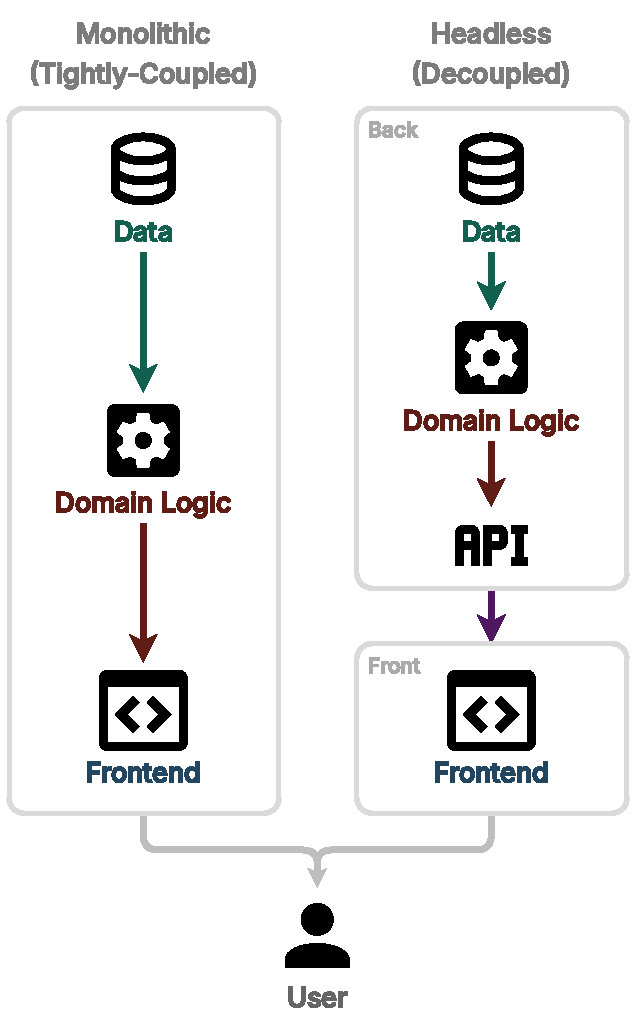
\includegraphics[width=0.65\textwidth]{web_arch_diff.pdf}
\end{figure}